% !TeX root = tikz-ext-manual.tex
% !TeX spellcheck = en_US
% Copyright 2022 by Qrrbrbirlbel
%
% This file may be distributed and/or modified
%
% 1. under the LaTeX Project Public License and/or
% 2. under the GNU Free Documentation License.
%

\section{Extending the Path Timers}
\label{library:timer}

\begin{tikzlibrary}{ext.paths.timer}
  This library adds timers to the path specifications |rectangle|, |parabola|, |sin| and |cos|.
  
  \inspiration{TimerRect-Q,TimerPara-Q}{TimerRect-A,TimerPara-A}
\end{tikzlibrary}

In \tikzname, the path specification |rectangle|, |parabola|, |sin| and |cos| do not provide
their own timer, i.\,e. a node placing algorithm that is dependent on the actual path.
For |rectangle| the timer of the straight line between the rectangle's corners is used, for
the other paths, nodes, coordinates, pics, etc. are placed on the last coordinate.

This library allows this.

\subsection{Rectangle}
\indexPathOperationO{rectangle}

For the |rectangle| path operator, the timer starts with |pos = 0| (= |at start|) from\indexKeyO{pos}
the starting coordinate in a counter-clockwise direction along the rectangle.
The corners will be at positions 0.0, 0.25, 0.5, 0.75 and 1.0.

\begin{key}{/\tikzext/rectangle timer=|line| or |rectangle|}
\keycompat{tikz}
By default, the library activates the new (correct) timer for |rectangle|.
With |rectangle timer = line| the original line timer can be reinstated.
\end{key}
\begin{codeexample}[width=10cm,preamble=\usetikzlibrary{ext.paths.timer}]
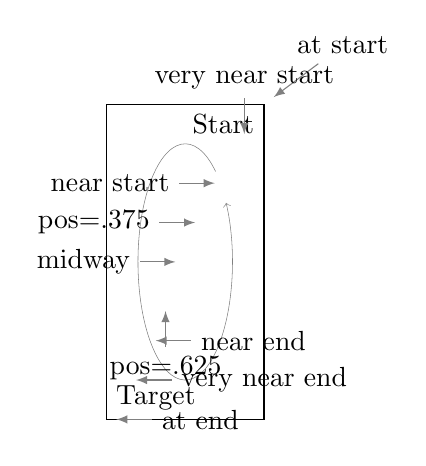
\begin{tikzpicture}[scale=2, every pin edge/.style={latex-, gray}]
\coordinate [label=above right:Target] (A) at (0,0);
\coordinate [label=below left:Start]   (B) at (1,2);
\draw[->, help lines] ([shift=(50:.3 and .75)] .5,1)
  arc[start angle=50, delta angle=340, x radius=.3, y radius=.75];
\draw (B) rectangle (A)
  foreach \pos/\ang in {at start/60, very near start/90, near start/180, pos=.375/180,
                        midway/180, pos=.625/270, near end/0, very near end/0, at end/0}{
    node[pin=\ang:\pos, style/.expanded=\pos]{}};
\end{tikzpicture}
\end{codeexample}

\subsection{Parabola}
\indexPathOperationO{parabola}%

For the |parabola| path operator the timer is similar to the |.. controls ..| operator.

The position 0.5 will lie at the |bend|.
\begin{codeexample}[width=.3\linewidth,preamble=\usetikzlibrary{ext.paths.timer}]
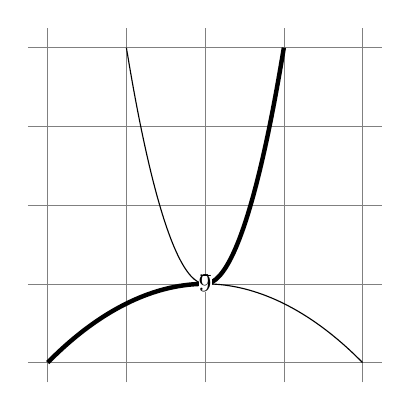
\begin{tikzpicture}
\draw[help lines]  (-2.25, -1.25) grid (2.25, 3.25);
\draw              ( 2,-1) parabola bend (0,0) (-1,3);
\draw[ultra thick] (-2,-1) parabola bend (0,0) ( 1,3)
  foreach \pos in {1,...,4,6,7,...,9}{
    node[
      pos=.\pos, sloped, fill=white, font=\small, inner sep=+0pt
    ] {\pos}
  };
\end{tikzpicture}
\end{codeexample}

If no |bend| is specified half the positions will collapse into one end of the curve.

\begin{codeexample}[width=.3\linewidth,preamble=\usetikzlibrary{ext.paths.timer}]
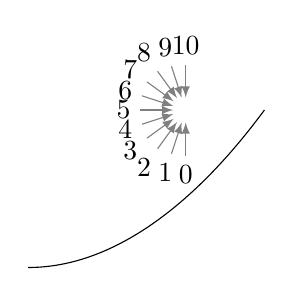
\begin{tikzpicture}[every pin edge/.style={latex-, shorten <=1pt, gray}]
\draw (-2,-2) parabola (1,0)
  foreach \pos in {0, 1, ..., 10} {
    node [pos=\pos/10, pin={[anchor=-18*\pos+90]-18*\pos+270:\pos}]{}
  };
\end{tikzpicture}
\end{codeexample}

\subsection{Sine/Cosine}
\indexPathOperationO{sin}\indexPathOperationO{cos}%

The |sin| and |cos| path operators also allow placing of nodes along their paths.

\begin{codeexample}[width=.3\linewidth,preamble=\usetikzlibrary{ext.paths.timer}]
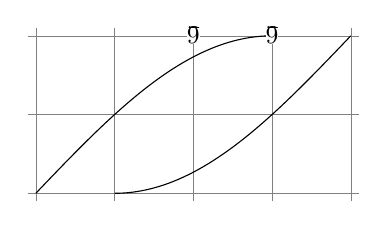
\begin{tikzpicture}[mark nodes on line/.style={insert path={
  foreach \pos in {1, ..., 9} {node[
    sloped, fill=white, font=\small, inner sep=+0pt, pos=\pos/10] {\pos}}}}]
\draw[help lines] (-2.1,-2.1) grid (2.1,0.1);
\draw             (-2,-2) sin (1,0) [mark nodes on line];
\draw[shift=(0:1)](-2,-2) cos (1,0) [mark nodes on line];
\end{tikzpicture}
\end{codeexample}
\endinput